% TEMPLATE for Usenix papers, specifically to meet requirements of
%  USENIX '05
% originally a template for producing IEEE-format articles using LaTeX.
%   written by Matthew Ward, CS Department, Worcester Polytechnic Institute.
% adapted by David Beazley for his excellent SWIG paper in Proceedings,
%   Tcl 96
% turned into a smartass generic template by De Clarke, with thanks to
%   both the above pioneers
% use at your own risk.  Complaints to /dev/null.
% make it two column with no page numbering, default is 10 point

% Munged by Fred Douglis <douglis@research.att.com> 10/97 to separate
% the .sty file from the LaTeX source template, so that people can
% more easily include the .sty file into an existing document.  Also
% changed to more closely follow the style guidelines as represented
% by the Word sample file. 

% Note that since 2010, USENIX does not require endnotes. If you want
% foot of page notes, don't include the endnotes package in the 
% usepackage command, below.

% This version uses the latex2e styles, not the very ancient 2.09 stuff.
\documentclass[letterpaper,twocolumn,10pt]{article}
\usepackage{usenix,epsfig,endnotes}
\usepackage[T1]{fontenc}
\begin{document}

%don't want date printed
\date{}

%make title bold and 14 pt font (Latex default is non-bold, 16 pt)
\title{\Large \bf Building a Modular ROS Network for the Raven II}

%for single author (just remove % characters)
\author{
{\rm Troy\ Sankey}\\
University of California Los Angeles
\and
{\rm Qu\ (Jackie)\ Jin}\\
University of California Los Angeles
\and
{\rm Jonathan\ Chan}\\
University of California Los Angeles
} % end author

% \maketitle

\twocolumn[
  \begin{@twocolumnfalse}
    \maketitle
    \begin{abstract}

The Raven II Surgical Robot is a 7-DOF cable-actuated surgical robot
designed for minimally invasive surgery and remote surgery. The robot
can be teleoperated by two Phantom Omnis, which are haptic devices
designed for medical training and research applications. The Raven
utilizes Robot Operating System (ROS), a collection of software
modules specially made for developing robot applications. Many
features of ROS could be beneficial to the the Raven, but are
inaccessible due to current code's limited use of ROS constructs. ROS
provides a comprehensive set of libraries and tools for developing
platform-independent robot applications, which is not fully utilized
in BRL's implementation. The current objective for the UCLA
development team is to fully integrate ROS into the Raven II which
would bring support for generic control, image processing, and basic
automation. This report covers the implementation of generic control
based on ROS.  \\\\

    \end{abstract}
  \end{@twocolumnfalse}
]


% Use the following at camera-ready time to suppress page numbers.
% Comment it out when you first submit the paper for review.
% \thispagestyle{empty}


\section{Introduction}
The Raven II surgical robotic arm was designed by the BioRobotics
Laboratory (BRL) at the University of Washington, and one copy of the
robot was given to the Center for Advanced Surgical and Interventional
Technology (CASIT) at the University of California Los Angeles to help
study and improve. Our team helped modularize the code base of the
Raven II as provided by BRL.

In computer science, using modular design guarantees code readability
and, most importantly, code shareability. The Raven II implements
Robot Operating System (ROS) which is a programming framework built
around the idea of modular components that are, in theory, so abstract
that they can even be shared across different robots. However, we
discovered that BRL's use of ROS programming constructs are minimal
(granted, ROS did not exist when the Raven was originally conceived).

\section{Motivation}

\subsection{Robots in MIS, and software}

\subsection{Understanding the Raven code}
The structure of the current raven system is straightfoward. At the
highest level, there is a master node and a slave node. The master
interprets the position and orientation of two Phantom Omni haptic
controllers (for both arms), translates them into a differential
position and orientation, then transmits that to the slave. The slave
will accumulate the differential pose\footnote{in robotics, \emph{pose}
  is the combination of position and orientation} into an absolute
pose, or goal pose, then attempt to reach the goal pose.

For the slave, this process repeats every millisecond. The master is
on its own time---there is no synchronization between the master and
slave.

The slave code spawns three threads:

\begin{itemize}
  \item console I/O
  \item networking
  \item control (e.g. IK, USB I/O)
\end{itemize}

The control thread is a realtime thread that, at a fixed interval,
updates its current and desired pose, calculates torques for each
motor, and applies those torques. This is referred to as the
\emph{control loop}, and can be seen in
\texttt{raven\_2/src/raven/rt\_process\_preempt.c}. 

\subsection{Lack of modular design in the Raven code}

\subsection{Image recognition}

\subsection{No-fly zones}

\subsection{Arbitrary controllers}

\section{Requirements}

\section{Design}

\begin{figure*}[ht!]
  \begin{center}
    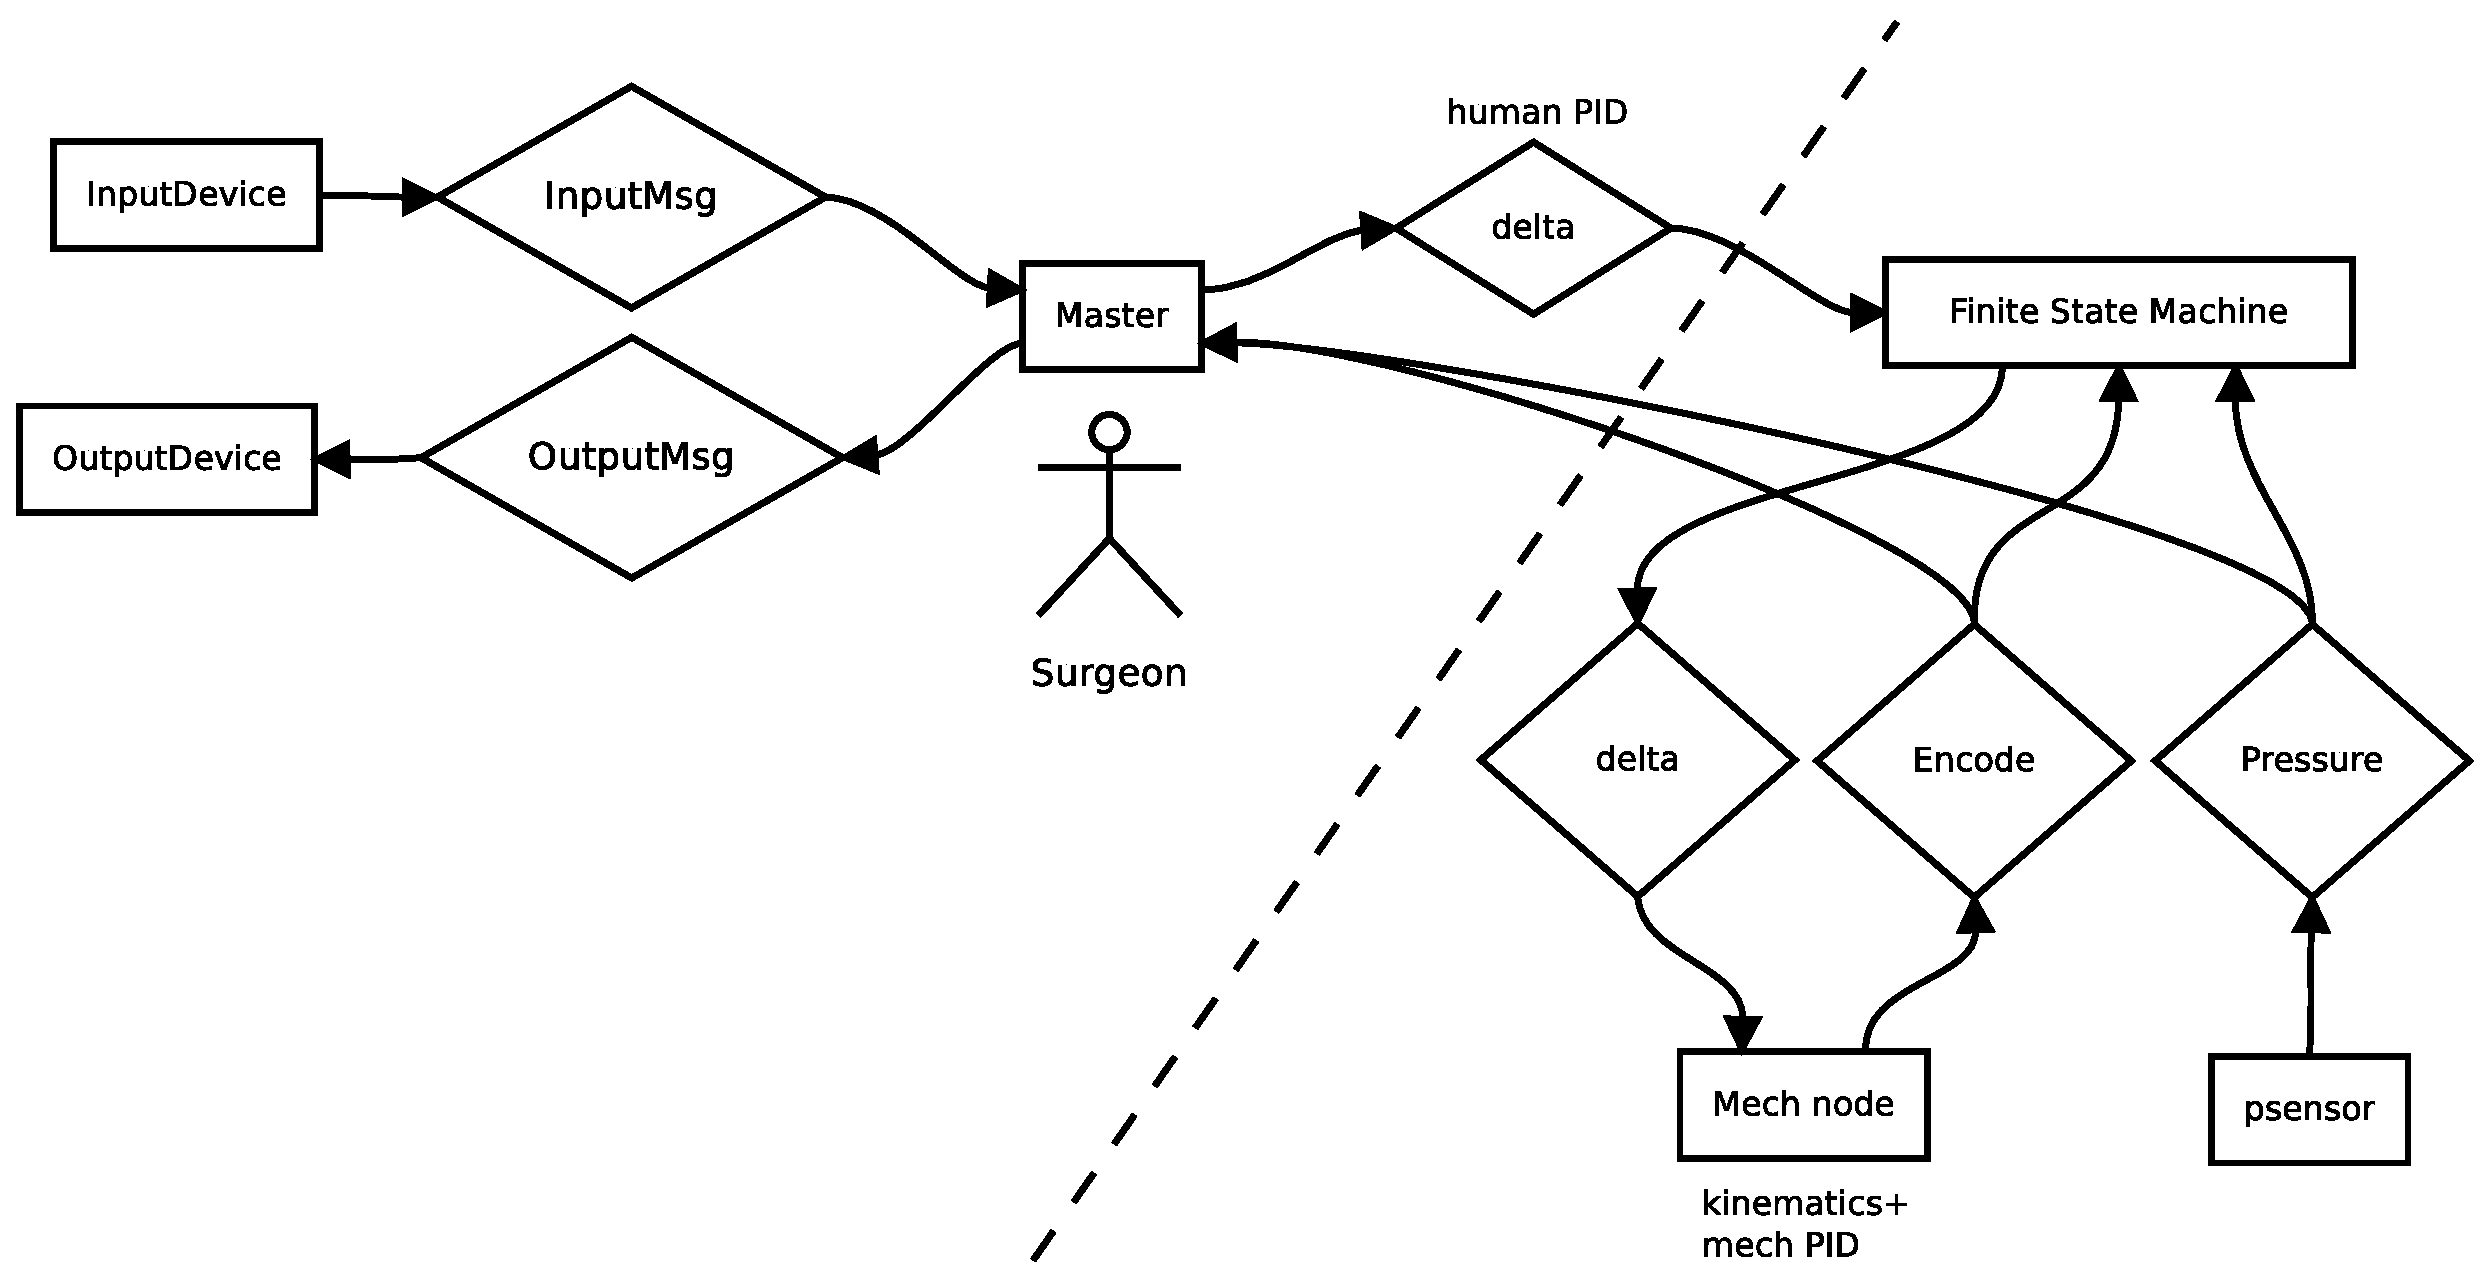
\includegraphics[width=1.0\textwidth]{ros_high_level_v2.eps}
  \end{center}
  \caption{Proposed ROS network for the Raven II. Everything to the
    left of the dashed line is \emph{master}, and everything to the
    right is \emph{slave}. Squares represent ROS nodes, diamonds
    represent ROS topics for passing messages.}
  \label{fig:ros_network}
\end{figure*}

Our top-level design of the ROS network replaces the \emph{networking}
thread, \emph{console I/O} thread, and the entire master side with ROS
components. The square Mech node in Figure ~\ref{fig:ros_network}
encasulates most of the existing raven code, including all of the code
responsible for gravity compensation, inverse kinematics, PID control,
and USB I/O. Our ROS network defines a standard interface between the
InputDevice node and the Master node, which would make implementing
new input devices straightforward---adding Wii Remote support or
LapaRobot support to the Raven should be straightforward since it
would not require knowledge of any part of the ROS network beyond its
interface with the Master node.

\subsection{Generic Control}

BRL hard-coded the control side as part of the Raven-II system so that
the control device can only be the Sensable Phantom Omni. Although the
Phantom Omni is a widely used haptic device for medical simulation and
training [2], such constraint would be a limiting factor for projects
involving other types of controllers. In our reimplementation, the
control node is contained within an independent ROS package called
{\it raven\_control}. It interacts with the finite state machine in
{\it raven\_fsm} through the ROS messaging system, as shown in Figure
1.

\begin{figure}
\includegraphics[scale=0.33]{ControlDiagram.jpg}
\caption{Controller-FSM Messaging}
\end{figure}

The {\it ControlDevice} node indicates the actual control device from
the user end. When the user triggers a control event, {\it
  ControlDevice} publishes the message (x, y, z, pitch, yaw, roll,
pedal and state) to the topic {\it raven/control}. On the subscriber
end, {\it ControlEmu} transforms the values of pitch, yaw and roll
into quaternion required by {\it raven\_mech}. The communication
between {\it ControlEmu} and the finite state machine is established
through a ROS service\footnote{ROS Services,
  http://www.ros.org/wiki/Services}. {\it ControlEmu} sends a request
to the service proxy which the finite state machine (FSM in short)
listens to. Once a control request is received, the FSM formulates a
message object and sends it to the topic {\it raven/fsm} subscribed by
the arm nodes (the arms are labeled "green" and "gold
respectively"). Once the arms are ready for next control event, the
FSM evaluates the situation and accordingly sends back a response to
{\it ControlEmu}. {\it ControlEmu} then issues a new request based on
the previous response.

Compared to the BRL's implementation, our implementation allows
generic control devices besides the Phantom Omni. The tested working
devices are keyboards, PlayStation3 controllers and generic PC game
controllers. Due to the incompleteness of the development, a control
device node needs to be manually added following the template in
Figure 2.

\begin{figure}
\includegraphics[scale=0.6]{ControlDeviceTemplate.png}
\caption{Control Device Python Template}
\end{figure}

Eventually users will be able to add and configure control devices
through either a {\it control.xml} file or a GTK
interface\footnote{GTK,http://www.gtk.org/}. The proper control nodes
will be generated based on the user input.

\subsection{Finite State Machine}

The finite state machine serves as a high-level commander of the
Raven-II system. It's in charge of the state estimation and
transition. Figure 3 shows the work flow of the FSM.

\begin{figure}
\includegraphics[scale=0.4]{FSM.png}
\caption{FSM Work Flow}
\end{figure}

After initialization, the FSM starts inspecting {\it raven\_mech}'s
homing action until it's done. The "Mode\_Switch" state is where major
estimation and transitions happen. Based on the user input, the FSM
transits to the corresponding state (control, sewing automation, tumor
tracking, etc). The current implementation leaves room for more modes
in the future development. Among all the modes, "Control" has the
highest priority. Any other modes can be interrupted by the user
control. This is a rather naive implementation mainly for testing and
is subject to change. Among all the states, "ESTOP/TERMINATION" has
the highest priority. The FSM goes to this state once there is an
emergency interruption. The FSM would then save the current state
record and properly stop the Raven-II system. The FSM is also designed
to communicate with external ROS nodes. Essentially modes can hand
work to ROS nodes and collect status for progress through
services. One example is the controller-FSM messaging mentioned in the
"Generic Control" section. If the "Control" mode is active, the FSM
communicates with {\it ControlEmu} through a service, gives {\it
  raven\_mech} orders through messages and reports to "Mode\_Switch"
for state estimation.

\section{Mistakes}

\section{Conclusion}


%% {\footnotesize \bibliographystyle{acm}
%% \bibliography{../common/bibliography}}

%% \theendnotes

\end{document}
